% These slides originally from Paul Goldsmith-Pinkham: https://github.com/paulgp

\documentclass[notes,11pt, aspectratio=169]{beamer}
\usetheme{metropolis}
\usepackage{pgfpages}
% These slides also contain speaker notes. You can print just the slides,
% just the notes, or both, depending on the setting below. Comment out the want
% you want.
\setbeameroption{hide notes} % Only slide
%\setbeameroption{show only notes} % Only notes
%\setbeameroption{show notes on second screen=right} % Both

\usepackage{helvet}
\usepackage[default]{lato}
\usepackage{array}


\usepackage{tikz}
\usepackage{verbatim}
\setbeamertemplate{note page}{\pagecolor{yellow!5}\insertnote}
\usetikzlibrary{positioning}
\usetikzlibrary{snakes}
\usetikzlibrary{calc}
\usetikzlibrary{arrows}
\usetikzlibrary{decorations.markings}
\usetikzlibrary{shapes.misc}
\usetikzlibrary{matrix,shapes,arrows,fit,tikzmark}
\usepackage{amsmath, amsfonts, amssymb, amsthm}
\usepackage{mathpazo}
\usepackage{hyperref}
\usepackage{lipsum}
\usepackage{multimedia}
\usepackage{multirow}
\usepackage{graphicx}
\usepackage{dcolumn}
\usepackage{bbm}
\newcolumntype{d}[0]{D{.}{.}{5}}
\graphicspath{{../../output/}}
\usepackage[]{epstopdf}
% This adds the output directory to the inputs function (code outputs are latex inputs!) so you don't have to use a relative path each time
\makeatletter
\providecommand*{\input@path}{}
\g@addto@macro\input@path{{../../output/}}% append
\makeatother


\usepackage{changepage}
\usepackage{appendixnumberbeamer}
\newcommand{\beginbackup}{
   \newcounter{framenumbervorappendix}
   \setcounter{framenumbervorappendix}{\value{framenumber}}
   \setbeamertemplate{footline}
   {
     \leavevmode%
     \hline
     box{%
       \begin{beamercolorbox}[wd=\paperwidth,ht=2.25ex,dp=1ex,right]{footlinecolor}%
%         \insertframenumber  \hspace*{2ex} 
       \end{beamercolorbox}}%
     \vskip0pt%
   }
 }
\newcommand{\backupend}{
   \addtocounter{framenumbervorappendix}{-\value{framenumber}}
   \addtocounter{framenumber}{\value{framenumbervorappendix}} 
}
\usepackage[space]{grffile}
\usepackage{booktabs}

\definecolor{blue}{RGB}{0,114,178}
\definecolor{red}{RGB}{213,94,0}
\definecolor{yellow}{RGB}{240,228,66}
\definecolor{green}{RGB}{0,158,115}
\definecolor{white}{RGB}{255,255,255}

\hypersetup{
  colorlinks=false,
  linkbordercolor = {yellow},
  linkcolor = {blue}
}


\definecolor{MyBackground}{RGB}{255,255,255}
\definecolor{MyTransition}{RGB}{86,180,233}
%% Uncomment this if you want to change the background color to something else
\setbeamercolor{background canvas}{bg=MyBackground}

%% Change the bg color to adjust your transition slide background color!
\newenvironment{transitionframe}{
  \setbeamercolor{background canvas}{bg=MyTransition}
  \begin{frame}}{
    \end{frame}
}

\setbeamercolor{frametitle}{fg=white}
\setbeamercolor{title}{fg=black}
\setbeamertemplate{footline}[frame number]
\setbeamertemplate{navigation symbols}{} 
\setbeamertemplate{itemize items}{-}
\setbeamercolor{itemize item}{fg=blue}
\setbeamercolor{itemize subitem}{fg=blue}
\setbeamercolor{enumerate item}{fg=blue}
\setbeamercolor{enumerate subitem}{fg=blue}
\setbeamercolor{button}{bg=MyBackground,fg=blue,}



% If you like road maps, rather than having clutter at the top, have a roadmap show up at the end of each section 
% (and after your introduction)
% Uncomment this is if you want the roadmap!
% \AtBeginSection[]
% {
%    \begin{frame}
%        \frametitle{Roadmap of Talk}
%        \tableofcontents[currentsection]
%    \end{frame}
% }
\setbeamercolor{section in toc}{fg=blue}
\setbeamercolor{subsection in toc}{fg=red}
\setbeamersize{text margin left=1em,text margin right=1em} 

\newenvironment{wideitemize}{\itemize\addtolength{\itemsep}{10pt}}{\enditemize}

\title[]{\textcolor{blue}{Title of the paper}}
\author[AET]{}
\institute[]{
\small{
	\begin{center}
		\begin{tabular}{cccc}
			Author  A& Author B & Author C & Author D \\
 			\multicolumn{4}{c}{Place}  \\
			\multicolumn{4}{c}{} \\
		  	\multicolumn{4}{c}{Author E}  \\
		 	\multicolumn{4}{c}{Place 2}
		\end{tabular}
	\end{center}
}}

\date[\today]{}


\begin{document}

%%% TIKZ STUFF
\tikzset{   
        every picture/.style={remember picture,baseline},
        every node/.style={anchor=base,align=center,outer sep=1.5pt},
        every path/.style={thick},
        }
\newcommand\marktopleft[1]{%
    \tikz[overlay,remember picture] 
        \node (marker-#1-a) at (-.3em,.3em) {};%
}
\newcommand\markbottomright[2]{%
    \tikz[overlay,remember picture] 
        \node (marker-#1-b) at (0em,0em) {};%
}
\tikzstyle{every picture}+=[remember picture] 
\tikzstyle{mybox} =[draw=black, very thick, rectangle, inner sep=10pt, inner ysep=20pt]
\tikzstyle{fancytitle} =[draw=black,fill=red, text=white]
%%%% END TIKZ STUFF

% Title Slide
\begin{frame}
\maketitle
  \centering{Caveats and disclaimers.}
  \thispagestyle{empty}
\end{frame}

\begin{frame}{Alternative co-author table}
	\large{
		\begin{center}
				
			\begin{tabular}{cccc}
				Author A$^*$ & Author B$^*$ & Author C$^*$ & Author D$^{\dagger,*}$ \\
				\multicolumn{4}{c}{} \\
				\multicolumn{4}{c}{\small{*: place 1;  $\dagger$: place 2}} 
			\end{tabular}
		\end{center}
	}
\end{frame}

% INTRO
\begin{frame}{Two columns}
\begin{columns}[T] % align columns
\begin{column}{.3\textwidth}
  \begin{wideitemize}
    \item Bullet point
  \end{wideitemize}
\end{column}%
\hfill%
\begin{column}{.7\textwidth}
  \makebox[\linewidth][c]{
    \resizebox{1.2\linewidth}{!}{
      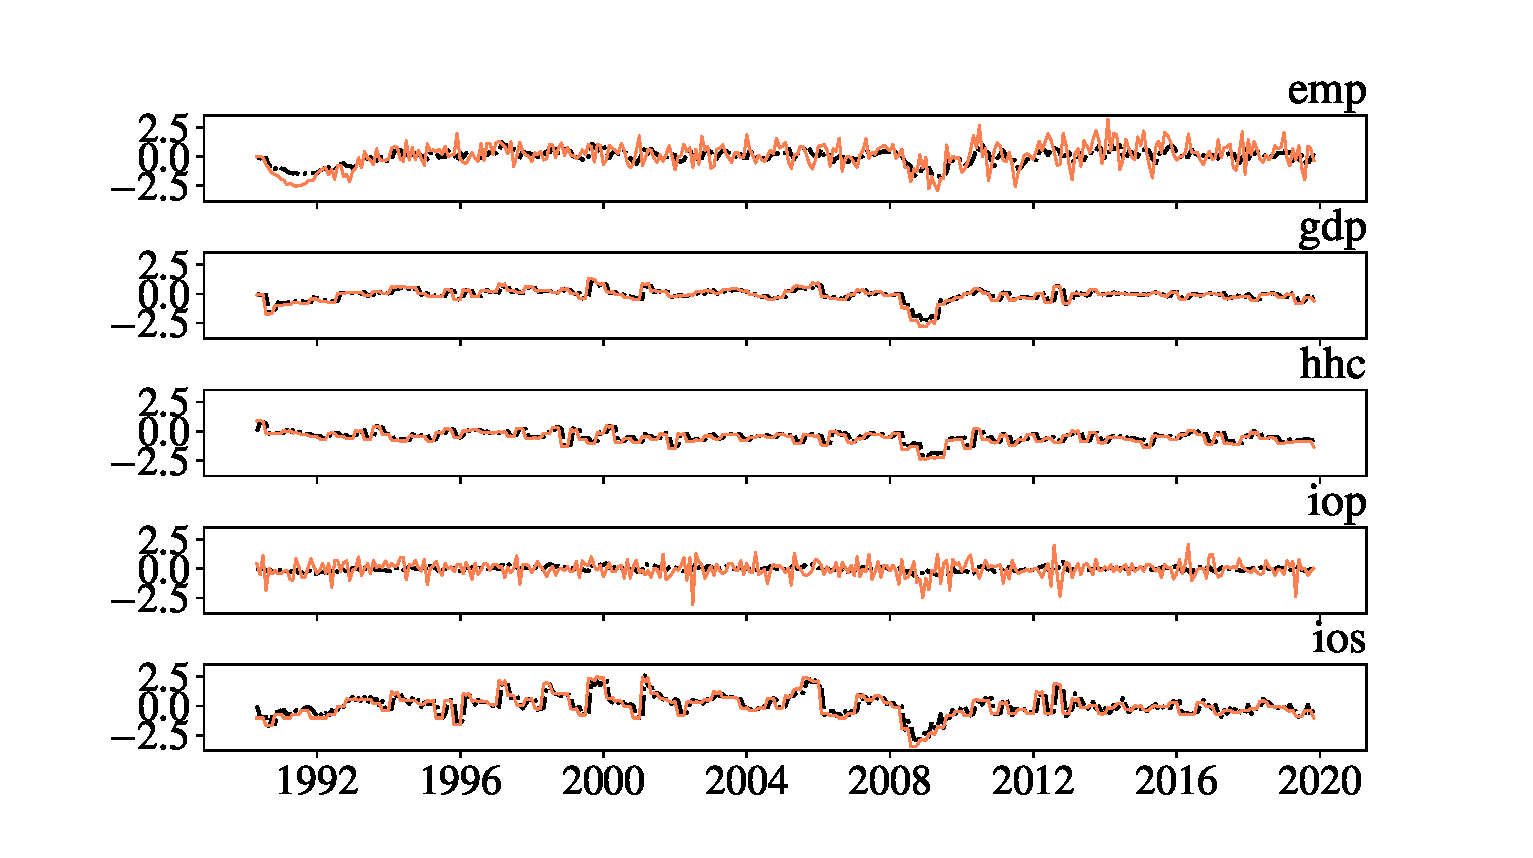
\includegraphics{fcasts.eps}
    }
  }
\end{column}%
\end{columns}
\end{frame}

\begin{frame}{Just bullets}
  \begin{wideitemize}
    \item $E = \gamma mc^2$
    \item ${\displaystyle {\frac {\partial p_{s}}{\partial t}}+{\vec {v}}\cdot {\vec {\nabla }}p_{s}+{\frac {Z_{s}e}{m_{s}}}\left({\vec {E}}+{\vec {v}}\times {\vec {B}}\right)\cdot {\vec {\nabla }}_{v}p_{s}=-{\frac {\partial }{\partial v_{i}}}\left(p_{s}\langle \Delta v_{i}\rangle \right)+{\frac {1}{2}}{\frac {\partial ^{2}}{\partial v_{i}\,\partial v_{j}}}\left(p_{s}\langle \Delta v_{i}\,\Delta v_{j}\rangle \right)}$
  \end{wideitemize}
\end{frame}

\begin{frame}{Just equations}
The model, it has the following specification:
$$
\begin{aligned} \vec{y}_t & = \Gamma \vec{f}_t + \vec{u}_t \\\\ 
        \vec{f}_t & = A_1 \vec{f}_{t-1} + A_2\vec{f}_{t-2} + \Xi_t \quad \quad \Xi_t \thicksim \mathcal{N}(0,I)\\\\ 
	 \vec{u}_t  & = B_1 \vec{u}_{t-1} + B_2\vec{u}_{t-2} + \Phi_t \quad \quad \Phi_t \thicksim \mathcal{N}(0,\Sigma)
\end{aligned}
$$
where capital Greek and Latin characters represent matrices, arrows over characters denote vectors, and it is assumed that the different components of the `innovations' in the error updating equation are uncorrelated so that $ \Sigma $ is a diagonal matrix. The model has one unobserved factor that follows an AR(2), and the errors similarly follow an AR(2).
\end{frame}



\section{Section}

\begin{transitionframe}
  \begin{center}
    { \Huge Transition frame}
  \end{center}
\end{transitionframe}

\begin{frame}{Just a figure}
  \makebox[\linewidth][c]{
    \resizebox{\linewidth}{!}{
      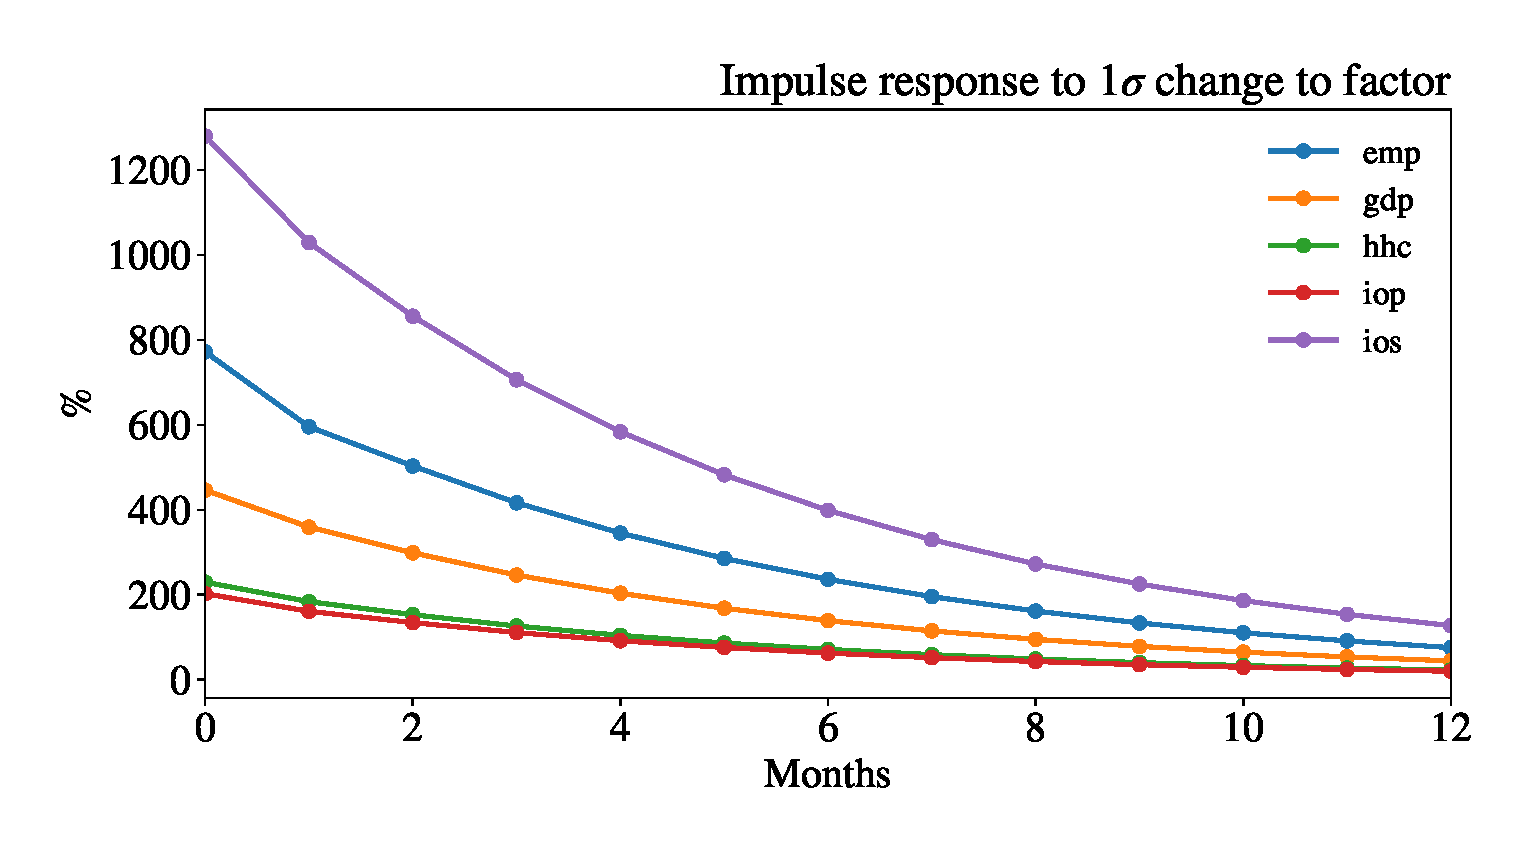
\includegraphics{df_irfs.eps}
    }
  }
\end{frame}

\begin{frame}{Input tex, e.g. tables, from elsewhere}
  \makebox[\linewidth][c]{
    \resizebox{\linewidth}{!}{
     \begin{center}
\begin{tabular}{lclc}
\toprule
\textbf{Dep. Variable:}          & ['emp', 'gdp', 'hhc', 'iop', 'ios'] & \textbf{  No. Observations:  } &                 355                  \\
\textbf{Model:}                  &  DynamicFactor(factors=2, order=2)  & \textbf{  Log Likelihood     } &              -2122.477               \\
\textbf{}                        &            + AR(2) errors           & \textbf{  AIC                } &               4310.955               \\
\textbf{Date:}                   &           Thu, 09 Jan 2020          & \textbf{  BIC                } &               4438.735               \\
\textbf{Time:}                   &               23:13:06              & \textbf{  HQIC               } &               4361.789               \\
\textbf{Sample:}                 &              04-30-1990             & \textbf{                     } &                                      \\
\textbf{}                        &             - 10-31-2019            & \textbf{                     } &                                      \\
\bottomrule
\end{tabular}
\begin{tabular}{lcccccc}
                          & \textbf{coef} & \textbf{std err} & \textbf{z} & \textbf{P$>$$|$z$|$} & \textbf{[0.025} & \textbf{0.975]}  \\
\midrule
\textbf{loading.f1.emp}   &       7.7198  &        1.081     &     7.143  &         0.000        &        5.602    &        9.838     \\
\textbf{loading.f2.emp}   &      -0.5070  &        0.428     &    -1.184  &         0.236        &       -1.346    &        0.332     \\
\textbf{loading.f1.gdp}   &       4.4642  &        0.332     &    13.441  &         0.000        &        3.813    &        5.115     \\
\textbf{loading.f2.gdp}   &       0.2476  &        0.232     &     1.065  &         0.287        &       -0.208    &        0.703     \\
\textbf{loading.f1.hhc}   &       2.2967  &        0.334     &     6.873  &         0.000        &        1.642    &        2.952     \\
\textbf{loading.f2.hhc}   &       0.0905  &        0.122     &     0.740  &         0.459        &       -0.149    &        0.330     \\
\textbf{loading.f1.iop}   &       2.0257  &        0.382     &     5.297  &         0.000        &        1.276    &        2.775     \\
\textbf{loading.f2.iop}   &       0.0417  &        0.112     &     0.371  &         0.710        &       -0.178    &        0.262     \\
\textbf{loading.f1.ios}   &      12.7989  &        0.806     &    15.881  &         0.000        &       11.219    &       14.378     \\
\textbf{loading.f2.ios}   &       0.6643  &        0.659     &     1.008  &         0.314        &       -0.628    &        1.957     \\
\textbf{sigma2.emp}       &       0.0367  &        0.294     &     0.125  &         0.901        &       -0.540    &        0.613     \\
\textbf{sigma2.gdp}       &       0.0303  &        0.004     &     7.658  &         0.000        &        0.023    &        0.038     \\
\textbf{sigma2.hhc}       &       0.1247  &        0.007     &    18.216  &         0.000        &        0.111    &        0.138     \\
\textbf{sigma2.iop}       &       0.4116  &        0.026     &    15.985  &         0.000        &        0.361    &        0.462     \\
\textbf{sigma2.ios}       &       0.0225  &        0.020     &     1.122  &         0.262        &       -0.017    &        0.062     \\
\textbf{L1.f1.f1}         &       0.7897  &       26.066     &     0.030  &         0.976        &      -50.299    &       51.878     \\
\textbf{L1.f2.f1}         &       0.0331  &        1.871     &     0.018  &         0.986        &       -3.634    &        3.700     \\
\textbf{L2.f1.f1}         &       0.0284  &       31.461     &     0.001  &         0.999        &      -61.634    &       61.691     \\
\textbf{L2.f2.f1}         &      -0.0108  &        1.917     &    -0.006  &         0.995        &       -3.769    &        3.747     \\
\textbf{L1.f1.f2}         &       0.2779  &        2.187     &     0.127  &         0.899        &       -4.009    &        4.564     \\
\textbf{L1.f2.f2}         &       0.3943  &        0.171     &     2.304  &         0.021        &        0.059    &        0.730     \\
\textbf{L2.f1.f2}         &      -0.1851  &        2.271     &    -0.081  &         0.935        &       -4.636    &        4.266     \\
\textbf{L2.f2.f2}         &       0.0310  &        0.194     &     0.160  &         0.873        &       -0.349    &        0.411     \\
\textbf{L1.e(emp).e(emp)} &       0.5036  &        2.372     &     0.212  &         0.832        &       -4.146    &        5.153     \\
\textbf{L2.e(emp).e(emp)} &       0.3334  &        2.111     &     0.158  &         0.875        &       -3.805    &        4.472     \\
\textbf{L1.e(gdp).e(gdp)} &       0.9721  &        0.128     &     7.624  &         0.000        &        0.722    &        1.222     \\
\textbf{L2.e(gdp).e(gdp)} &      -0.1488  &        0.119     &    -1.253  &         0.210        &       -0.382    &        0.084     \\
\textbf{L1.e(hhc).e(hhc)} &       0.9047  &        0.142     &     6.353  &         0.000        &        0.626    &        1.184     \\
\textbf{L2.e(hhc).e(hhc)} &      -0.0635  &        0.141     &    -0.450  &         0.653        &       -0.340    &        0.213     \\
\textbf{L1.e(iop).e(iop)} &      -0.1792  &        0.056     &    -3.222  &         0.001        &       -0.288    &       -0.070     \\
\textbf{L2.e(iop).e(iop)} &      -0.0587  &        0.053     &    -1.101  &         0.271        &       -0.163    &        0.046     \\
\textbf{L1.e(ios).e(ios)} &       0.2006  &        0.133     &     1.509  &         0.131        &       -0.060    &        0.461     \\
\textbf{L2.e(ios).e(ios)} &       0.7877  &        0.145     &     5.419  &         0.000        &        0.503    &        1.073     \\
\bottomrule
\end{tabular}
\begin{tabular}{lclc}
\textbf{Ljung-Box (Q):}          & 75.96, 61.07, 150.64, 50.14, 33.55 & \textbf{  Jarque-Bera (JB):  } & 3.70, 16.59, 325.28, 54.11, 1250.25  \\
\textbf{Prob(Q):}                &    0.00, 0.02, 0.00, 0.13, 0.75    & \textbf{  Prob(JB):          } &     0.16, 0.00, 0.00, 0.00, 0.00     \\
\textbf{Heteroskedasticity (H):} &    2.43, 2.38, 0.90, 1.28, 0.60    & \textbf{  Skew:              } &   0.22, -0.07, -0.02, -0.42, 0.80    \\
\textbf{Prob(H) (two-sided):}    &    0.00, 0.00, 0.58, 0.18, 0.01    & \textbf{  Kurtosis:          } &    3.23, 4.05, 7.69, 4.71, 12.05     \\
\bottomrule
\end{tabular}
%\caption{Statespace Model Results}
\end{center}

Warnings: \newline
 [1] Covariance matrix calculated using the outer product of gradients (complex-step). \newline
 [2] Covariance matrix is singular or near-singular, with condition number 3.19e+16. Standard errors may be unstable.
    }
  }
\end{frame}



\section{Appendix}
\begin{transitionframe}
  \begin{center}
    \Huge Appendix!
  \end{center}
\end{transitionframe}


\appendix

\begin{frame}[label=appendix_start]{Backup slides}
  \begin{wideitemize}
  \item Backup slide land \hyperlink{appendix_end}{\beamergotobutton{Next slide}}
  \end{wideitemize}
\end{frame}

\begin{frame}[label=appendix_end]{And switch back}
  \begin{wideitemize}
      \item[]  Go back buttons \hyperlink{appendix_start}{\beamergotobutton{Back}}
  \end{wideitemize}
\end{frame}



\end{document}
